% Created 2013-10-14 Lun 00:09
\documentclass[bigger,hyperref={colorlinks=true, urlcolor=red, plainpages=false, pdfpagelabels, bookmarksnumbered}]{beamer}
\usepackage[utf8]{inputenc}
\usepackage[T1]{fontenc}
\usepackage{fixltx2e}
\usepackage{graphicx}
\usepackage{longtable}
\usepackage{float}
\usepackage{wrapfig}
\usepackage{soul}
\usepackage{textcomp}
\usepackage{marvosym}
\usepackage{wasysym}
\usepackage{latexsym}
\usepackage{amssymb}
\usepackage{hyperref}
\tolerance=1000
\usepackage{color}
\usepackage{listings}
\AtBeginSection[]{\begin{frame}<beamer>\frametitle{Table of Contents}\tableofcontents[currentsection]\end{frame}}
\lstset{
keywordstyle=\color{blue},
commentstyle=\color{red},
stringstyle=\color{green},
basicstyle=\ttfamily\small,
columns=fullflexible,
frame=single,
basewidth={0.5em,0.4em}
}
\RequirePackage{fancyvrb}
\DefineVerbatimEnvironment{verbatim}{Verbatim}{fontsize=\small,formatcom = {\color[rgb]{0.5,0,0}}}
\providecommand{\alert}[1]{\textbf{#1}}

\title{IMW: Middleware}
\author{Stephane Genaud}
\date{\today}
\hypersetup{
  pdfkeywords={},
  pdfsubject={},
  pdfcreator={Emacs Org-mode version 7.9.3f}}

\usetheme{Boadilla}\usecolortheme{default}
\setbeamertemplate{footline}{\leavevmode \hbox{ \begin{beamercolorbox}[wd=.6\paperwidth,ht=2.25ex,dp=1ex,center]{title in head/foot} \insertshorttitle\end{beamercolorbox} \begin{beamercolorbox}[wd=.25\paperwidth,ht=2.25ex,dp=1ex,center]{date in head/foot}\insertshortauthor\end{beamercolorbox} \begin{beamercolorbox}[wd=.15\paperwidth,ht=2.25ex,dp=1ex,right]{title in head/foot} \insertframenumber / \inserttotalframenumber\hspace*{2em} \end{beamercolorbox} } \vskip0pt }
\setbeamercovered{invisible}
\author[S. Genaud]{{\large Stéphane Genaud} \\ \vspace{0.2cm} ENSIIE - Strasbourg \\ \vspace{0.2cm} \texttt{genaud@unistra.fr} }
\date{{\large Middleware} \\ \vspace{0.2cm} }
\begin{document}

\maketitle

\begin{frame}
\frametitle{Outline}
\setcounter{tocdepth}{3}
\tableofcontents
\end{frame}









\section{Introduction}
\label{sec-1}
\begin{frame}
\frametitle{Technologies for Distributed Systems}
\label{sec-1-1}

\begin{itemize}
\item Extremely fast evolution since 1985:
     about a technology every 5 years.\\
\item Implementations adapt to up-to-date technology\\
e.g If networks go faster, it is possible to convey bigger messages.\\
         If the cost of some hardware becomes low, no need to spare it.
\end{itemize}
\end{frame}
\begin{frame}
\frametitle{Technologies change but \ldots{} concepts stay}
\label{sec-1-2}

\begin{itemize}
\item Client-server is the central concept:\\
The \textbf{client} can make a request at any time,\\
      The \textbf{server} permanently waits for incoming requests
\end{itemize}
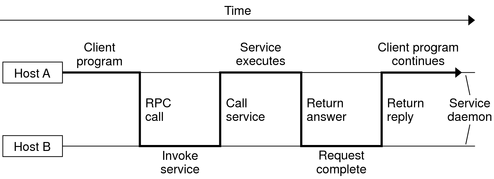
\includegraphics[width=.9\linewidth]{./img/S9_RPC_works.png}
\end{frame}
\begin{frame}
\frametitle{Middleware: definition}
\label{sec-1-3}
\begin{block}{What is middleware?}
\label{sec-1-3-1}

\begin{itemize}
\item A sofware layer between the OS and the application allowing 
      a set of distributed computers to communicate in a standardized
      way.
\end{itemize}
\end{block}
\begin{itemize}

\item Middleware provides inter-machines communication facilities,\\
\label{sec-1-3-2}%
but may also include services, such as authentification services,
    resource directories, distributed file catalogs, \ldots{}
     
\end{itemize} % ends low level
\end{frame}
\begin{frame}
\frametitle{A Time-line of technologies}
\label{sec-1-4}

  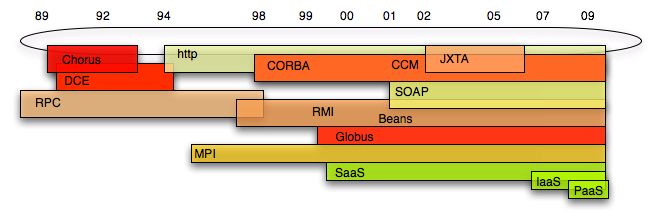
\includegraphics[width=.9\linewidth]{../img/timeline.png}
\end{frame}
\begin{frame}
\frametitle{Principle Design Choices}
\label{sec-1-5}

\begin{itemize}
\item Abstraction vs. Performance
\item Interoperability
\item Versatility
\end{itemize}
\end{frame}
\begin{frame}
\frametitle{Abstraction}
\label{sec-1-6}
\begin{itemize}

\item Abstraction of communication primitives
\label{sec-1-6-1}%
\begin{itemize}
\item too low level: rapidly obsolete, lower programming productivity
\item too high level: difficult to optimize for performance
\end{itemize}

\item Abstraction Trade-off
\label{sec-1-6-2}%
\begin{itemize}
\item independent from the architecture: execute across
      different systems without \textbf{source code} modification
\item Hide details related to communication/synchronization management
      (e.g \texttt{Remote Procedure Calls} more abstract than \texttt{sockets})
\end{itemize}
                                          
\end{itemize} % ends low level
\end{frame}
\begin{frame}
\frametitle{Interoperability}
\label{sec-1-7}
\begin{itemize}

\item Machine-independent\\
\label{sec-1-7-1}%
e.g \href{http://www.ietf.org/rfc/rfc1057.txt}{Sun RPC} 
    \vspace{5mm}

\item OS-independent\\
\label{sec-1-7-2}%
e.g \href{http://www.oracle.com/technetwork/java/javase/tech/index-jsp-136424.html}{Java-RMI}
    \vspace{5mm}

\item Language-independent\\
\label{sec-1-7-3}%
e.g \href{http://www.corba.org}{Corba}, \href{http://www.w3.org/TR/soap/}{SOAP}
\end{itemize} % ends low level
\end{frame}
\begin{frame}
\frametitle{Versatility}
\label{sec-1-8}

   The more general, the more versatile 
\begin{itemize}
\item Example 1: SOAP communicates through XML pieces of text
\item $\Rightarrow$ SOAP toolkits can be found for almost all languages.
\end{itemize}
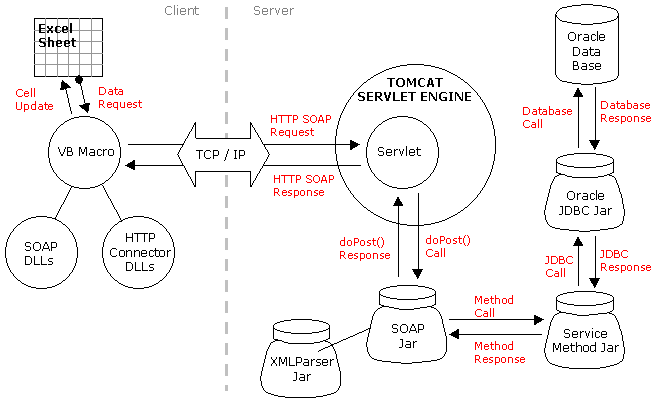
\includegraphics[width=.9\linewidth]{../soap-img/soapuser-archi1.png}
\end{frame}
\section{Sun RPC}
\label{sec-2}
\begin{frame}
\frametitle{Background}
\label{sec-2-1}

   Sun RPC  (aka RPC ONC (Open Network Computing)) 
\begin{itemize}
\item are the original RPC (\href{http://tools.ietf.org/html/rfc1831}{RFC 1831}), introduced by Sun in 1988
\item motivation: provide a support to inter-machines services
\item NFS as first target, NIS, \ldots{}.
\item is open source software (BSD license since 2009)
\end{itemize}
\end{frame}
\begin{frame}
\frametitle{Interoperability}
\label{sec-2-2}

\begin{itemize}
\item ONC RPC allow programs on different OS and machines to communicate
\item It may be in different languages but C in 99\% cases.
\item Relies on \href{http://www.ietf.org/rfc/rfc4506.txt}{XDR} (eXternal Data Representation)
\end{itemize}
     
\end{frame}
\begin{frame}[fragile]
\frametitle{RPC service identification}
\label{sec-2-3}
\begin{block}{Services are identified by}
\label{sec-2-3-1}

\begin{enumerate}
\item the program name (\verb~prog_name~)
\item the program version (\verb~prog_ver~)
\item the function name
\end{enumerate}
\end{block}
\begin{beamercolorbox}{Example}
\label{sec-2-3-2}


\lstset{language=C}
\begin{lstlisting}
program MYPROG {
  version VERSION_ONE {
    void MYPROG_NULL(void) = 0;
    answer MYPROG_MYFUNC(data) = 1;
  } = 1;
} = 0x2000:0001;
\end{lstlisting}
 
\end{beamercolorbox}
\end{frame}
\begin{frame}
\frametitle{Service Registration (portmap)}
\label{sec-2-4}

 This service must be registered in a directory service generally called \emph{portmapper} 
\begin{itemize}
\item acts as a name server
\item converts : <prog$_{\mathrm{name}}$ + ver + protocol> to <portnumber>
\item exact service name depending on sytem/distribution : \texttt{rpcbind} (or sometimes \texttt{portmap}, or \texttt{rpc.portmap})
\item attached to port 111
\end{itemize}
\end{frame}
\begin{frame}[fragile]
\frametitle{Standard RPC services}
\label{sec-2-5}
\begin{block}{file \texttt{/etc/rpc}}
\label{sec-2-5-1}


\lstset{language=C}
\begin{lstlisting}
portmapper  100000  
rstatd      100001  
rusersd     100002  
nfs         100003  
ypserv      100004 
mountd      100005 
ypbind      100007
walld       100008
\end{lstlisting}
     
\end{block}
\end{frame}
\begin{frame}[fragile]
\frametitle{Running Services}
\label{sec-2-6}


\lstset{language=C}
\begin{lstlisting}
  % rpcinfo -p
    program vers proto   port
   100000    2   tcp    111  portmapper
   100000    2   udp    111  portmapper
536870913    1   udp  58764
536870913    1   tcp  65106
\end{lstlisting}
 Two last lines are one user program.


 
\end{frame}
\begin{frame}
\frametitle{Programming with ONC RPC}
\label{sec-2-7}

   Two layers:
\begin{itemize}

\item The \textbf{higher} layer: small set of functions to describe and call services in a simple way.
\label{sec-2-7-1}%
\begin{itemize}
\item Essential primitives: \texttt{registerrpc()} and \texttt{callrpc()} \\
\item However, limitations: udp only, no auth, and encoding/decoding by hand.
\end{itemize}


\item The \textbf{lower} layer: 20+ functions to fine tune the calls.
\label{sec-2-7-2}%
\begin{itemize}
\item Much more complex, used for stressed services, for example 
     to implement asynchronous RPC and authentification.
\end{itemize}

\end{itemize} % ends low level
\end{frame}
\begin{frame}
\frametitle{Server-side steps}
\label{sec-2-8}

   The server must \textbf{register}: asks the local portmap to:
\begin{enumerate}
\item create a new entry so that clients can be routed
\item associate a service number and the address of the function 
     that implements it, or the address of the \emph{dispatcher}.
\end{enumerate}
\begin{itemize}

\item The primtives are
\label{sec-2-8-1}%
\begin{itemize}
\item \texttt{svc\_register()} and \texttt{pmap\_set()} (low level)
\item \texttt{rpcregister()} (high level)
\item on exit, \texttt{svc\_unregister()}, \texttt{pmap\_uset()}
\end{itemize}
\end{itemize} % ends low level
\end{frame}
\begin{frame}
\frametitle{Client-side steps}
\label{sec-2-9}

   The client must initialize (1), lookup in remote portmap to find the service (2),
   then, several calls can be made afterwards (3):
\begin{enumerate}
\item \texttt{clnt\_create()} / \texttt{clnttcp\_create()} / \texttt{clntudp\_create()},
\item \texttt{pmap\_getport()}
\item \texttt{clnt\_call()}
\end{enumerate}

   The higher level \texttt{callrpc()} does steps 1, 2 and 3 in a row.
\end{frame}
\begin{frame}[fragile]
\frametitle{Example of high-layer usage (server side 1/2)}
\label{sec-2-10}

\emph{Define the service on the server:}

\lstset{language=C}
\begin{lstlisting}
#include <rpc/xdr.h>
#include <rpc/rpc.h>

int* my_function(int *n) {
   static int res;
   *n = *n + 1;
   res= *n; 
   return (&res);
}
\end{lstlisting}
 
\end{frame}
\begin{frame}[fragile]
\frametitle{Example of high-layer usage (server side 2/2)}
\label{sec-2-11}

\emph{Register the service on the server:}

\lstset{language=C}
\begin{lstlisting}
#define PROGNUM 0x20000100                                                      
#define VERSNUM 1                                                               
#define PROCNUM 1

int main (void) {
   registerrpc( PROGNUM,
                VERSNUM,
                PROCNUM,
                my_function, /*ptr to function*/
                (xdrproc_t) xdr_int, /*encode input*/
                (xdrproc_t) xdr_int);/*decode output*/

    svc_run(); /*  server starts listening ... */
}
\end{lstlisting}
\end{frame}
\begin{frame}[fragile]
\frametitle{Example of high-layer usage (client side 1/2)}
\label{sec-2-12}

   \emph{Call the service from the client:}

\lstset{language=C}
\begin{lstlisting}
int main (int argc, char **argv) {
 int n=0x41424344;
 char *host = argv[1];
 int stat;
 stat = callrpc(host,
                PROGNUM,
                VERSNUM,
                PROCNUM,
                (xdrproc_t) xdr_int, //intput encoding
                (char *)&n,          //input param
                (xdrproc_t)xdr_int,  //output decoding
                (char *)&res);       //return of func
}
\end{lstlisting}
 
\end{frame}
\begin{frame}
\frametitle{Another way: \texttt{rpcgen}}
\label{sec-2-13}

\begin{itemize}
\item Taking care of conversion through XDR is difficult
\item The \texttt{rpcgen} compiler automates the process of writing RPC applications
\item \texttt{rpcgen} accepts interface descriptions in \href{http://docs.oracle.com/cd/E19683-01/816-1435/6m7rrfn9k/index.html}{RPCL (RPC Language)}
\item and generates skeletons programs (C code)
\end{itemize}
\end{frame}
\begin{frame}[fragile]
\frametitle{Example with \texttt{rpcgen}}
\label{sec-2-14}

\begin{itemize}
\item Consider an \emph{operation} \texttt{addition}, that adds up 2 \texttt{int} s
\item Describe this service in a file \texttt{myservice.x}
\end{itemize}

\lstset{language=C}
\begin{lstlisting}
struct data {
  int arg1;  int arg2;
};
typedef struct data data;
struct response {
  int result; unsigned char error;
};
typedef struct response response;

program MYCOMPUTATION {
  version VERSION_ONE{
    void MYCOMPUTATION_NULL(void) = 0;
    response MYCOMPUTATION_ADDITION(data) = 1;
  } = 1;
} = 0x20000001;
\end{lstlisting}
\end{frame}
\begin{frame}[fragile]
\frametitle{Example with \texttt{rpcgen} (contd)}
\label{sec-2-15}

\begin{itemize}
\item Generate the skeletons
\end{itemize}

\lstset{language=C}
\begin{lstlisting}
% rpcgen -a myservice.x
\end{lstlisting}
\begin{itemize}
\item The following files are generated
\end{itemize}

\lstset{language=C}
\begin{lstlisting}
myservice.h        /* parameter definitions */
myservice_xdr.c    /* XDR conversion */
myservice_svc.c    /* stubs server */   
myservice_clnt.c   /* stubs client */
myservice_server.c /* server code */
myservice_client.c /* client code */
\end{lstlisting}
\end{frame}
\begin{frame}[fragile]
\frametitle{RPCL in Brief (enumeration, constants \& simple)}
\label{sec-2-16}
\begin{itemize}

\item Enumerations and Constants\\
\label{sec-2-16-1}%
\lstset{language=C}
\begin{lstlisting}
enum colortype { RED = 0, GREEN = 1,BLUE = 2  };
const PI = 3.14;
\end{lstlisting}

\item Simple Declarations\\
\label{sec-2-16-2}%
\lstset{language=C}
\begin{lstlisting}
int length;
colortype c;
\end{lstlisting}

\item Added types (bool and string)
\label{sec-2-16-3}%
\begin{itemize}
\item \texttt{bool} : boolean, can take TRUE or FALSE values
\item \texttt{string}: translated to \texttt{char *} (See variable length array).
\end{itemize}
\end{itemize} % ends low level
\end{frame}
\begin{frame}[fragile]
\frametitle{RPCL in Brief (arrays)}
\label{sec-2-17}
\begin{itemize}

\item Fixed-length arrays\\
\label{sec-2-17-1}%
\lstset{language=C}
\begin{lstlisting}
int length[5];
color palette[8];
\end{lstlisting}


\item Variable-length arrays
\label{sec-2-17-2}%
\begin{itemize}
\item The maximum size is specified between angle brackets, or may be ommitted:
\end{itemize}

\lstset{language=C}
\begin{lstlisting}
int notes_serie<20>;   # at most 20
int heights<>;         # unlimited
string message<256>;
\end{lstlisting}
each will translate to a C struct, e.g:

\lstset{language=C}
\begin{lstlisting}
struct {
   u_int heights_len;/* # of items in array */
   int *heights_val; /* pointer to array */
} heights;
\end{lstlisting}
\end{itemize} % ends low level
\end{frame}
\begin{frame}[fragile]
\frametitle{RPCL in brief (typedef)}
\label{sec-2-18}
\begin{itemize}

\item Type definitions\\
\label{sec-2-18-1}%
Same syntax as C typedef

\lstset{language=C}
\begin{lstlisting}
typedef string name_t<255>; 
typedef string longstring<>;
\end{lstlisting}
will be translated into C code:

\lstset{language=C}
\begin{lstlisting}
typedef char *name_t;
typedef char *longstring;
\end{lstlisting}

\end{itemize} % ends low level
\end{frame}
\begin{frame}[fragile]
\frametitle{RPCL in Brief (pointers)}
\label{sec-2-19}

\begin{itemize}
\item Pointer declarations are as in C. Address pointers are not sent over the network. 
     Instead, data pointed to are copied. This is useful for sending recursive data 
     types such as lists and trees.
\end{itemize}

\lstset{language=C}
\begin{lstlisting}
tree_t *t;
\end{lstlisting}
\end{frame}
\begin{frame}[fragile]
\frametitle{RPCL in Brief (struct)}
\label{sec-2-20}

\begin{itemize}
\item Translates as is in C, excepted that an extra typedef is generated.
\end{itemize}

\lstset{language=C}
\begin{lstlisting}
struct coord {  int x;  int y;  };
\end{lstlisting}
Translates to:

\lstset{language=C}
\begin{lstlisting}
struct coord {  int x;  int y;  };
typedef struct coord coord;
\end{lstlisting}
which allows to use \texttt{coord} instead of \texttt{struct coord}
\end{frame}
\begin{frame}
\frametitle{Tips \& Tricks}
\label{sec-2-21}
\begin{block}{Linux}
\label{sec-2-21-1}

\begin{itemize}
\item Install: rpc lib provided by package  \texttt{libtirpc-dev}  (0.2.2-5 on ubuntu 12.04)
\item Run: a portmapper is provided by package \texttt{rpcbind}
\item Run: \texttt{svc\_register()} might refuse to register (``credentials problem'') 
           $\Rightarrow$ Start server as root or in sudo mode.
\item Initialize array variables before calling remote functions 
     (``Can't encode arguments'' error).
\end{itemize}
\end{block}
\begin{block}{MacOSX}
\label{sec-2-21-2}

\begin{itemize}
\item Install: the `Command line tools' element from Xcode in the distrib
              or download it fom  \href{https://developer.apple.com/downloads/}{Apple} .
\item Use: \texttt{rpcgen -C} to force generation of ANSI-C code
\end{itemize}
   
\end{block}
\end{frame}
\section{Java RMI}
\label{sec-3}
\begin{frame}
\frametitle{History}
\label{sec-3-1}

\begin{itemize}
\item Created by Sun in 1998
\item Java only
\item Available since JDK >= 1.1
\item Since JDK 1.5, stubs are automatically generated (no \texttt{rmic})
\end{itemize}
\end{frame}
\begin{frame}
\frametitle{RPC in the world of RMI}
\label{sec-3-2}

\begin{itemize}
\item RMI provides access to \textbf{objects} and their \textbf{methods}
\item In contrast to Sun RPC, not only data can be passed
     to remote computations, but also objects that can contain
     code and data.\\[5mm]
\item There are 2 ways to communicate in this object-oriented
     paradigm:
\begin{enumerate}
\item through the \texttt{Remote} class
\item through the \texttt{Serializable} class
\end{enumerate}
\end{itemize}
\end{frame}
\begin{frame}
\frametitle{The Remote class}
\label{sec-3-3}

   
   definition: An object of the Remote class can be used remotely.
   It can be used:
\begin{itemize}
\item in the address space of the JVM that created it,
\item in the address spaces of other JVMs through \emph{handles} (aka \emph{proxies}).
\end{itemize}
   
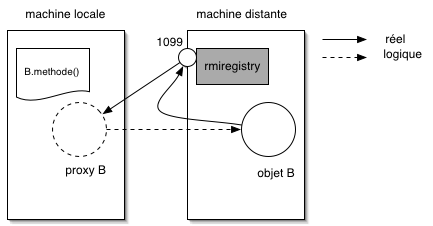
\includegraphics[width=.9\linewidth]{../img/proxy.png}
The call to a remote object's method is exactly (syntactically) the same as a local one.   
\end{frame}
\begin{frame}[fragile]
\frametitle{The Remote class  and interface}
\label{sec-3-4}
\begin{itemize}

\item A Remote class must be defined in 2 parts
\label{sec-3-4-1}%
\begin{itemize}
\item an interface
\item the class itself
\end{itemize}
\end{itemize} % ends low level
\begin{block}{Interface}
\label{sec-3-4-2}


\lstset{language=java}
\begin{lstlisting}
public interface MyExample extends Remote {...}
\end{lstlisting}
    
\end{block}
\begin{block}{Class}
\label{sec-3-4-3}


\lstset{language=java}
\begin{lstlisting}
public class MyExampleImpl 
  extends    UnicastRemoteObject
  implements MyExample  {
    ...
   }
\end{lstlisting}
\end{block}
\end{frame}
\begin{frame}
\frametitle{The Serializable class}
\label{sec-3-5}


definition: an object of the class Serializable is an object
that can be copied from one address space to another.
\end{frame}
\begin{frame}
\frametitle{Registering the services}
\label{sec-3-6}

   A process called \textbf{rmiregistry} is in charge of service registration\\
   (Equivalent of portmapper)
\begin{block}{Characteristics of \texttt{rmiregistry}}
\label{sec-3-6-1}

\begin{itemize}
\item runs on the same host as the services
\item default port is 1099
\item can be started by program
\end{itemize}
\end{block}
\end{frame}
\begin{frame}
\frametitle{Example 1: Remote object with primitive types}
\label{sec-3-7}

Example parameter passing using primitive types (e.g. int, float, ..) or arrays (e.g. String) 
\begin{itemize}
\item In general, parameters just need to be \textbf{serializable} (java.io.Serializable).
\end{itemize}
\begin{block}{The different pieces of code}
\label{sec-3-7-1}

\begin{itemize}
\item The service: description of the function prototype
\item The service: the implementation of the service
\item The server: a generic code which registers the service
\item The client: the code that uses the service
\end{itemize}
\end{block}
\end{frame}
\begin{frame}[fragile]
\frametitle{Example 1: Service Description}
\label{sec-3-8}


A service is described by an \textbf{interface}.
\begin{itemize}
\item known by the client and the server.
\end{itemize}
 

\lstset{language=java}
\begin{lstlisting}
import java.rmi.Remote;
import java.rmi.RemoteException;

public interface Operation extends Remote {

    public int addition(int a, int b) 
                    throws RemoteException ;
}
\end{lstlisting}
\end{frame}
\begin{frame}[fragile]
\frametitle{Example 1: Service Implementation}
\label{sec-3-9}

\begin{itemize}
\item Only the server \textbf{implements} the service.
\end{itemize}

\lstset{language=java}
\begin{lstlisting}
import java.rmi.server.UnicastRemoteObject ;
import java.rmi.RemoteException ;
import java.net.InetAddress.* ;
import java.net.* ;

public class OperationImpl extends UnicastRemoteObject
  implements Operation  {

    public OperationImpl () throws RemoteException {
        super();
    };

    public int addition(int a, int b) 
                    throws RemoteException {
      return( a + b) ;
  }
}
\end{lstlisting}
\end{frame}
\begin{frame}[fragile]
\frametitle{Example 1: Service Registration}
\label{sec-3-10}

\begin{itemize}
\item The first server task is to register the service 
  in the rmiregistry under a name (here \emph{Operation})
\end{itemize}

\lstset{language=java}
\begin{lstlisting}
import java.rmi.*;
import java.net.*;

public class Serveur {
  public static void main(String [] args) {
    try {
       OperationImpl une_op = new OperationImpl ();
       Naming.rebind("rmi://"+args[0]+"/Operation",une_op) ;
       System.out.println("Serveur pret");
     }
     catch (Exception e) { 
           System.out.println(re) ; 
     }
}
\end{lstlisting}
\end{frame}
\begin{frame}[fragile]
\frametitle{Example 1: Client code}
\label{sec-3-11}

\begin{itemize}
\item gets a reference to the  the service in the registry (proxy)
\item call the service using that reference
\end{itemize}


\lstset{language=java}
\begin{lstlisting}
import java.rmi.* ;
import java.net.MalformedURLException ;
import java.io.*;

public class Client {
  public static void main(String [] args) {
    try {
         Operation o = (Operation) 
             Naming.lookup("//"+args[0]+"/Operation");
         System.out.println("Client: 33+45= ?");
         int r = o.addition( 33, 45 );
         System.out.println("33+45="+ r );
     }
     catch (Exception e) { System.out.println(e) ; }
   }
}
\end{lstlisting}
\end{frame}
\begin{frame}[fragile]
\frametitle{Trouble shooting 1}
\label{sec-3-12}
\begin{block}{Observation}
\label{sec-3-12-1}

    The client experiences a \texttt{connection refused} error when 
    contacting the server.
\end{block}
\begin{block}{Why?}
\label{sec-3-12-2}

    \texttt{\$JAVA\_HOME/lib/security/java.policy} is too restrictive wrt sockets
\end{block}
\begin{block}{Solution}
\label{sec-3-12-3}

   To override the standard, run

\lstset{language=java}
\begin{lstlisting}
java -Djava.security.policy=more_perm Server
\end{lstlisting}
   where \texttt{fichier} contains, for instance:

\lstset{language=java}
\begin{lstlisting}
grant {
    permission java.net.SocketPermission
    "*:80-65535","connect,accept,listen,resolve";
    permission java.security.AllPermission;
};
\end{lstlisting}
   
\end{block}
\end{frame}
\begin{frame}[fragile]
\frametitle{Trouble shooting 2}
\label{sec-3-13}
\begin{block}{Observation}
\label{sec-3-13-1}

   When calling the RPC (hence after the lookup), the client ends with:
   \texttt{java.rmi.ConnectException: Connection refused to host: 127.0.0.1}
\end{block}
\begin{block}{Why?}
\label{sec-3-13-2}

   In some linux distributions, the name resolution for hostname
   takes 127.0.0.1 from \texttt{/etc/hosts} instead of public IP.
\end{block}
\begin{block}{Solution}
\label{sec-3-13-3}

run the server by overriding its IP

\lstset{language=java}
\begin{lstlisting}
java -Djava.rmi.server.hostname=<my ip here> Server
\end{lstlisting}
\end{block}
\end{frame}
\section{Corba}
\label{sec-4}
\begin{frame}
\frametitle{History}
\label{sec-4-1}
\begin{itemize}

\item Context
\label{sec-4-1-1}%
\begin{itemize}
\item A specification defined by the \emph{Object Management Group} (OMG), 
     composed of about 1000 members
\item currently CORBA 3.0
\item Implementors then propose implementations
\end{itemize}


\item Implemenations\\
\label{sec-4-1-2}%
Commercial :
\begin{itemize}
\item ORBIS, IONA, VisiBroker, ORBacus, \ldots{}.
\end{itemize}
     Open source:
\begin{itemize}
\item JDK, MICO, JacORB, TAO, \ldots{}
\end{itemize}

\end{itemize} % ends low level
\end{frame}
\begin{frame}
\frametitle{Characteristics}
\label{sec-4-2}


CORBA = Common Object Request Broker Architecture
\begin{itemize}

\item A RPC framework
\label{sec-4-2-1}%
\begin{itemize}
\item object oriented
\item multiple-OS, multiple languages can be involved
\item analogy of the ``software bus''
\end{itemize}

\item External Services
\label{sec-4-2-2}%
\begin{itemize}
\item helper services, can connect to the bus
\item services: naming, transaction, persistence \ldots{}
\end{itemize}

\end{itemize} % ends low level
\end{frame}
\begin{frame}
\frametitle{IDL}
\label{sec-4-3}


   The Interface Definition Language:
   equivalent to the RPC Language.

\begin{itemize}
\item defines the \textbf{methods} a server proposes
\item defines the \textbf{data} that can be accessed from the client (get/set)
\end{itemize}

   From IDL, generation of concrete code to
   represent data and methods in the chosen language.
 
\end{frame}
\begin{frame}[fragile]
\frametitle{IDL structure}
\label{sec-4-4}


Three hierarchical elements:
\begin{enumerate}
\item \texttt{Module} : namespaces (correspond to Java packages)
\item \texttt{Interface} : logical groups of methods
\item \emph{methods} : prototypes of the methods implemented by the server
\end{enumerate}

Example:

\lstset{language=idl}
\begin{lstlisting}
module HelloApp
{
  interface Hello
  {
  string sayHello();
  oneway void shutdown();
  };
};
\end{lstlisting}
\end{frame}
\begin{frame}
\frametitle{IDL types}
\label{sec-4-5}

Types and number of bytes between parenthesis: 
\begin{itemize}
\item boolean =\{TRUE,FALSE\}
\item octet (1)
\item \emph{signed} : short (2), long (4), long long (8)
\item \emph{unsigned} : unsigned short (2), unsigned long (4), unsigned long long (8)
\item \emph{floats} : float (4), double (8), long double (16)
\item \emph{characters}: char (1, iso-latin-1), string (var), string<n> (n), wchar (2, unicode), wstring (var of wchar)
\end{itemize}
\end{frame}
\begin{frame}
\frametitle{IDL type mapping to Java}
\label{sec-4-6}



\begin{center}
\begin{tabular}{lllll}
 IDL          &  Java    &     &  IDL                 &  Java    \\
\hline
 octet        &  byte    &     &  unsigned short      &  short   \\
 short        &  short   &     &  unsigned long       &  int     \\
 long         &  int     &     &  unsigned long long  &  long    \\
 long long    &  long    &     &  char                &  char    \\
 float        &  float   &     &  wchar               &  char    \\
 double       &  double  &     &  string              &  String  \\
 long double  &  N/A     &     &  wstring             &  String  \\
\end{tabular}
\end{center}
\end{frame}
\begin{frame}
\frametitle{IDL Methods}
\label{sec-4-7}
\begin{block}{General Form}
\label{sec-4-7-1}

<return$_{\mathrm{type}}$> method$_{\mathrm{name}}$([<mode> <type> <parameter$_{\mathrm{id}}$>]*) [raises [exceptions]+]; 

\begin{itemize}
\item mode=\{in, out, inout\} for input, output, and modified parameters resp.
\item type: all primitive or constructed type with typedef (constructed before method call)
\end{itemize}

Method names must be unique (no overloading).
\end{block}
\end{frame}
\begin{frame}
\frametitle{POA}
\label{sec-4-8}
\begin{block}{OA and POA}
\label{sec-4-8-1}

\begin{itemize}
\item Object Adapter: mechanism that connects a request using an object reference with
\end{itemize}
the proper code to service that request. 

\begin{itemize}
\item Portable Object Adapter: a particular type of object adapter that is 
  defined by the CORBA specification.
\end{itemize}
\end{block}
\begin{itemize}

\item characteristics
\label{sec-4-8-2}%
\begin{itemize}
\item Enables portability of object implementations between different ORB products
\item Provide support for objects with persistent identities
\item Provide support for transparent activation of objects
\item Allow a single servant to support multiple object identities simultaneously
\end{itemize}


\end{itemize} % ends low level
\end{frame}

\end{document}
